\documentclass{article}

\usepackage{graphicx}
\usepackage{tikz}
\usepackage{tikzsymbols}
\usetikzlibrary{calc,patterns,shapes.geometric}
\pagestyle{empty}
\usepackage[margin=0pt]{geometry}
\geometry{papersize={14in,12in}}

\def\centerarc[#1](#2)(#3:#4:#5){\draw[#1] ($(#2)+({#5*cos(#3)},{#5*sin(#3)})$) arc (#3:#4:#5);}

\begin{document}
	\begin{figure}
		\centering
		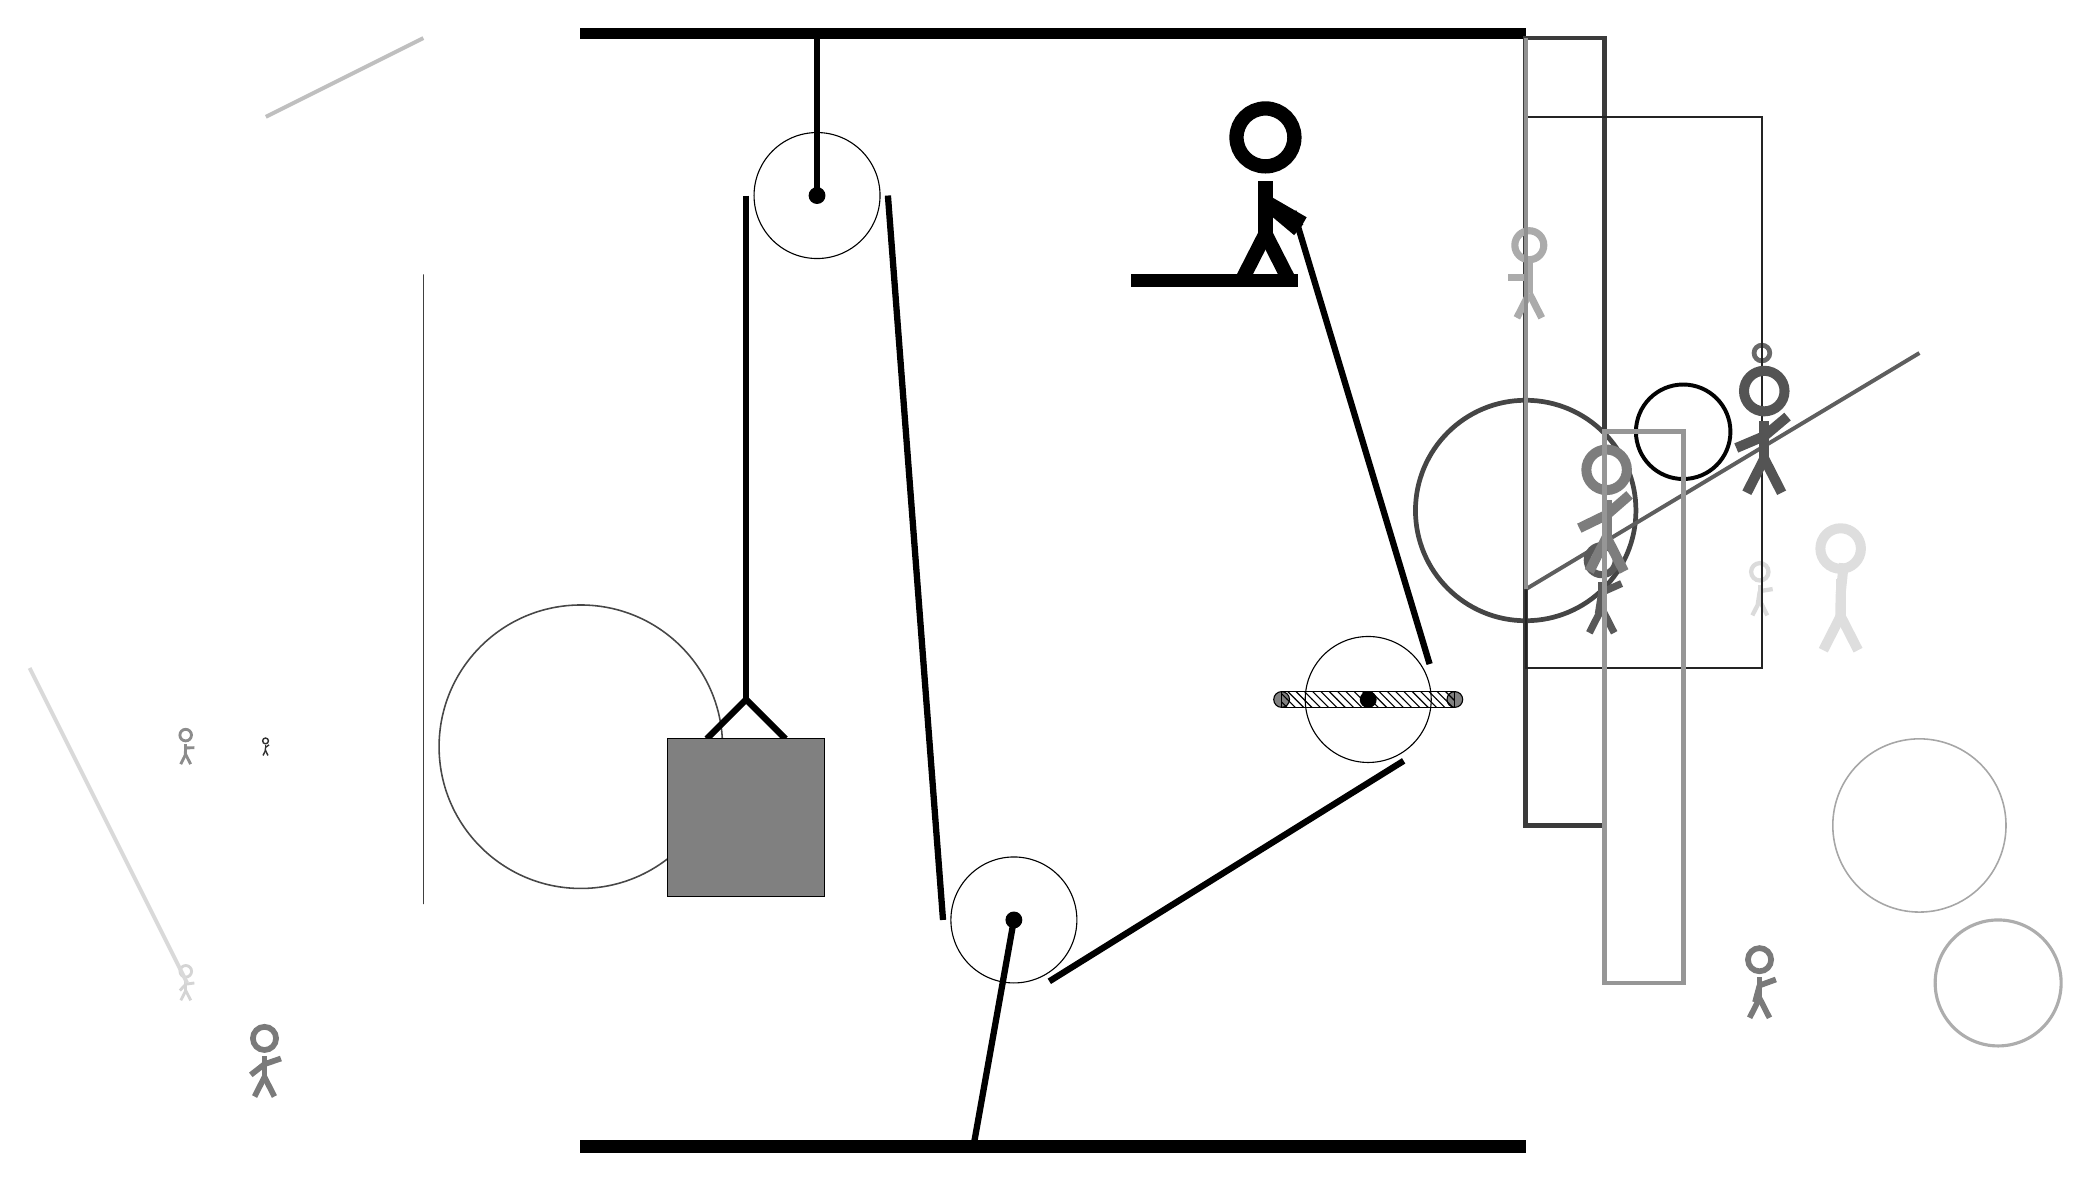
\begin{tikzpicture}
			%%%%% START %%%%%
			
			\draw[fill=black] (-2, 14) rectangle (10, 14.125);
			
			\draw (1, 12) circle (0.8);
			\draw[fill=black] (1, 12) circle (0.1);
			\draw[line width=0.8mm] (1, 14) -- (1, 12);
			
			\draw [line width=0.2mm, color=black!72](-2, 5) circle (1.8);
			
			\draw[line width=0.5mm, color=black!25](-4, 14) -- (-6, 13);
			\node[line width=0.2mm, color=black!17] at (-7, 2) {\Strichmaxerl[2][47][8]};
			\node[line width=0.6mm, color=black!45] at (-7, 5) {\Strichmaxerl[2][86][2]};
			\draw [line width=0.6mm, color=black!73](10, 8) circle (1.4);
			
			\node[line width=0.4mm, color=black!14] at (13, 7) {\Strichmaxerl[3][81][9]};
			\draw[line width=0.5mm, color=black!63](10, 7) -- (15, 10);
			
			\draw [line width=0.6mm, color=black!59](13, 10) circle (0.1);
			\node[line width=0.6mm, color=black!52] at (13, 2) {\Strichmaxerl[4][75][20]};
			\draw [line width=0.4mm, color=black!32](16, 2) circle (0.8);
			\draw[line width=0.6mm, color=black!77] (10, 4) rectangle (11, 14);
			
			\node[line width=0.4mm, color=black!65] at (11, 7) {\Strichmaxerl[5][81][24]};
			\draw [line width=0.5mm, color=black!99](12, 9) circle (0.6);
			
			\draw[line width=0.2mm, color=black!86] (10, 13) rectangle (13, 6);
			\node[line width=0.6mm, color=black!33] at (10, 11) {\Strichmaxerl[5][0][90]};
			\draw[line width=0.5mm, color=black!43] (10, 14) rectangle (10, 7);
			
			\draw [line width=0.2mm, color=black!35](15, 4) circle (1.1);
			\node[line width=0.4mm, color=black!51] at (11, 8) {\Strichmaxerl[7][26][41]};
			\node[line width=0.7mm, color=black!67] at (13, 9) {\Strichmaxerl[7][23][40]};
			\draw[line width=0.5mm, color=black!15](-7, 2) -- (-9, 6);
			\node[line width=0.6mm, color=black!52] at (-6, 1) {\Strichmaxerl[4][38][19]};
			
			\node[line width=0.4mm, color=black!13] at (14, 7) {\Strichmaxerl[7][89][84]};
			
			\draw[line width=0.2mm, color=black!75] (-4, 11) rectangle (-4, 3);
			\draw[line width=0.6mm, color=black!41] (11, 9) rectangle (12, 2);
			\node[line width=0.2mm, color=black!81] at (-6, 5) {\Strichmaxerl[1][87][35]};
			
			
			\draw (3.5, 2.8) circle (0.8);
			\draw[fill=black] (3.5, 2.8) circle (0.1);
			\draw[line width=0.8mm] (3.5, 2.8) -- (3.0, 0);
			
			\draw[fill=white](8, 5.6) circle (0.8);
			\draw[fill=black] (8, 5.6) circle (0.1);
			\draw[fill=black!50] (9.1, 5.6) circle (0.1);
			\draw[fill=black!50] (6.9, 5.6) circle (0.1);
			\draw[pattern=north west lines, pattern color=black] (6.9, 5.7) rectangle (9.1, 5.5);
			
			\draw[line width=0.8mm](-0.4, 5.1) --  (0.1, 5.6) -- (0.6, 5.1);
			\draw[fill=black!50] (-0.9, 5.1) rectangle (1.1, 3.1);
			
			\draw[line width=0.8mm](0.1, 12) -- (0.1, 5.6);
			\centerarc[line width=0.8mm](1, 12)(180:0:0.9)
			\draw[line width=0.8mm](1.9, 12) -- (2.6, 2.8);
			\centerarc[line width=0.8mm](3.5, 2.8)(180:300:0.9);
			\draw[line width=0.8mm](3.95, 2.0206) -- (8.45, 4.8206);
			\centerarc[line width=0.8mm](8, 5.6)(300:390:0.9);
			\draw[line width=0.8mm](8.7794, 6.05) -- (7.05, 11.8);
			
			\node at (6.75, 12) {\Strichmaxerl[10][-220][-30]};
			\draw[fill=black] (5, 11) rectangle (7.1, 10.85);
			
			\draw[fill=black] (-2, 0) rectangle (10, -0.15);
			
			%%%%% END %%%%%
		\end{tikzpicture}
	\end{figure}	
\end{document}